\section{MWP-CWP}
\label{sec:mwp-cwp}

The MWP-CWP analytical model offers a novel approach to understanding the performance of GPU 
architectures by examining the parallelism exhibited by MWP and CWP. As multithreaded architectures, GPUs allow multiple warps 
to be executed concurrently on a streaming multiprocessor (SM), effectively hiding the execution 
costs of these warps. The MWP-CWP model focuses on determining the maximum number of warps that 
can access memory simultaneously and the number of warps that an SM processor can execute during 
a memory warp waiting period. By carefully analyzing the relationship between MWP and CWP, this 
model provides valuable insights into the factors that govern execution time, revealing whether 
it is dominated by computation or memory access costs. Through a series of illustrative cases, we 
will demonstrate the importance of sufficient warps and the intricate interplay between MWP and CWP 
in optimizing GPU performance.\cite{DBLP:conf/isca/HongK09,marcmwpcwpslides}

\begin{figure}[H]
	\centering % <-- added
	\begin{subfigure}[b]{0.55\textwidth}
        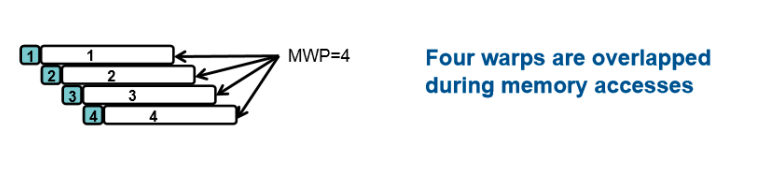
\includegraphics[width=\linewidth]{Figures/MWP.png}
        \caption{MWP}
        \label{fig:mwp}
	\end{subfigure}\hfil % <-- added
	\begin{subfigure}[b]{0.45\textwidth}
		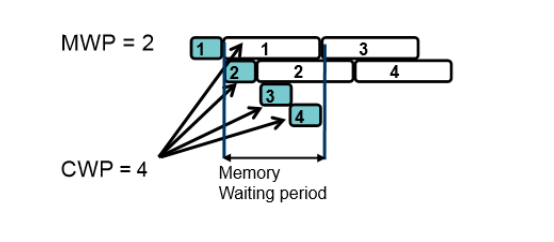
\includegraphics[width=\linewidth]{Figures/CWP.png}
	    \caption{CWP}
	    \label{fig:cwp}
	\end{subfigure}
	\label{fig:mwpcwpmodel}
    \caption{MWP-CWP model}
\end{figure}

\subsection{$MWP \leq CWP$}
\label{sec:mwp-cwp:1}

In the case where CWP is greater than MWP, the application's performance exhibits a distinct 
characteristic: computation cycles are effectively hidden by memory waiting periods. This implies 
that the computational resources are kept busy while the memory accesses are being processed, 
leading to a more efficient use of the available resources. However, the overall performance of 
the application is dominated by the memory cycles, as the computational work is executed in parallel 
with memory access operations. In other words, the system exhibits a higher degree of parallelism in 
computation than in-memory operations. This implies that while the application effectively utilizes 
the available computational resources, it may face limitations in leveraging memory-level parallelism. 
This imbalance between CWP and MWP can result in the underutilization of memory bandwidth and potentially 
lead to performance bottlenecks.\cite{DBLP:conf/isca/HongK09,marcmwpcwpslides}

\begin{figure}[htb]
    \centering
    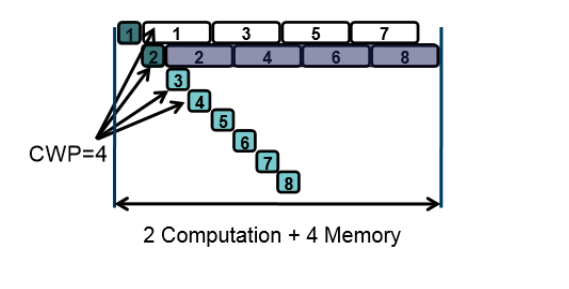
\includegraphics[width=0.65\linewidth]{Figures/cwpgreaterthanmwp.png}
	\caption{Computation cycles are concealed by memory waiting periods, 
             resulting in the overall performance being predominantly dictated by memory cycles.}
	\label{fig:cwpgreaterthanmwp}
\end{figure}

\subsection{$MWP > CWP$}
\label{sec:mwp-cwp:2}

In the scenario where MWP is greater than CWP, the application's performance demonstrates a contrasting behavior: 
memory accesses are predominantly hidden due to the high MWP. This means that the memory subsystem is capable 
of handling multiple memory requests concurrently while the computation resources are being utilized, 
effectively masking memory latencies. As a result, the overall performance of the application is dominated 
by the computation cycles, since the memory accesses are efficiently processed in parallel with the computational 
work. To put it differently, the application's performance may be hindered due to an imbalance between memory 
and computational resources. This disparity indicates that the application has a higher degree of parallelism 
in memory access than in computation, which can potentially result in the underutilization of computational 
resources.\cite{DBLP:conf/isca/HongK09,marcmwpcwpslides}

\begin{figure}[htb]
    \centering
    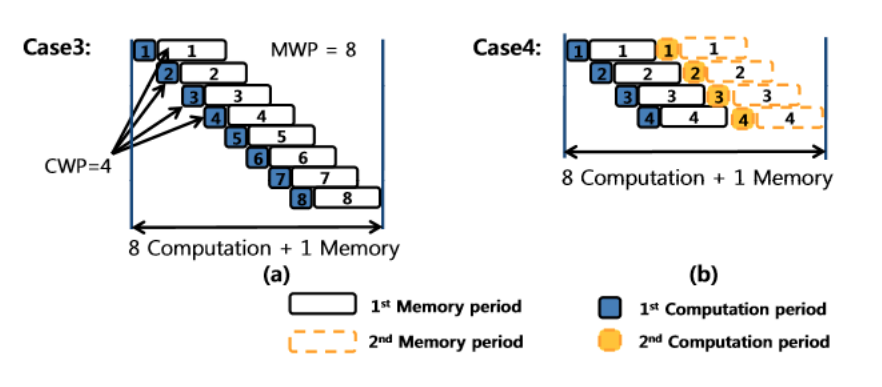
\includegraphics[width=0.65\linewidth]{Figures/mwpgreaterthancwp.png}
	\caption{Memory accesses are largely concealed by high MWP, 
            leading to the overall performance being primarily governed by computation cycles.}
	\label{fig:mwpgreaterthancwp}
\end{figure}
